\documentclass[11pt,a4paper]{article}

\usepackage[utf8]{inputenc}
\usepackage[T1]{fontenc}
\usepackage[english]{babel}
\usepackage{amsmath,amssymb}
\usepackage{graphicx}
\usepackage{booktabs}
\usepackage{caption}
\usepackage{geometry}
\usepackage{titling}
\usepackage{titlesec}
\usepackage[numbers,sort&compress]{natbib}
\usepackage[colorlinks=true,linkcolor=blue,citecolor=blue,urlcolor=blue]{hyperref}
\usepackage[textsize=footnotesize,textwidth=3cm]{todonotes}

\geometry{top=1.8cm,bottom=2.5cm,left=2.5cm,right=2.5cm}
\graphicspath{{aufgabe_02/figures/}}

% Compact layout: this is section 1/5 of the report, so keep it short --
% smaller, numbered citations; smaller captions; less space around headings and the title.
\setlength{\droptitle}{-2.2em}
\captionsetup{font=footnotesize,labelfont=bf,skip=4pt}
\renewcommand{\bibfont}{\footnotesize}
\titlespacing*{\section}{0pt}{1.4ex plus .2ex minus .2ex}{0.8ex plus .1ex}

% shorthand macros
\newcommand{\dr}{dimensionality reduction}
\newcommand{\tsne}{t-SNE}
\newcommand{\trust}{trustworthiness}
\newcommand{\knnp}{kNN-preservation}
\newcommand{\best}[1]{\textcolor{green!50!black}{\textbf{#1}}}
\newcommand{\worst}[1]{\textcolor{red}{#1}}

\title{Benchmark of comparative single-cell analysis approaches\\
\large Group-Project SSBI 2026}
\author{Sebastian Fay \and Marie Schygulla \and Gregor Habitzreither}
\date{September 2026}

\begin{document}
\maketitle

\section*{Introduction}
Analysing single-cell data brings some particular difficulties compared to bulk measurements: cells
from the same donor are not independent replicates of that donor's biology, and only a subset of a
donor's cells may show a phenotype of interest, so donor-level labels cannot simply be treated as
cell-level labels. In this project we compare and try to improve CellCnn \citep{arvaniti2017cellcnn}, an unsupervised representation-learning method developed to detect disease-associated cell subsets.

Our data come from Horowitz et al.\ \citep{horowitz2013nk} and cover 20 donors(9 CMV+, 11 CMV$-$), including 4 identifiable monozygotic twin pairs. Each donor's history of cytomegalovirus (CMV) infection was recorded, since CMV infection is known to leave behind a population of long-lived, memory-like ("adaptive") natural killer (NK) cells. This CMV label was assigned donor-wise, even though only a small subpopulation of that donor's NK cells actually carries the phenotypic signature linked to the infection. From each sample, 37 protein markers were measured by CyTOF, a technique that reads out metal-isotope-tagged antibodies via time-of-flight
mass spectrometry. Before subsampling, NK cells made up between 2.4\,\% and 16.2\,\% of alive events per donor.

To avoid a bias arising from donors contributing very different numbers of cells, we randomly selected
2{,}000 cells from each donor to obtain a balanced subsample. To check representativeness, we compared
the fraction of NKG2C$^+$/CD57$^+$ cells (a marker combination associated with the adaptive,
CMV-associated NK phenotype) in the balanced subsample against the fraction in the complete cell
population of each donor (Supp.\ Fig.~\ref{fig:subsample}): the subsample is representative for this
specific two-marker phenotype, though we did not check other marker combinations or rarer populations.

Before \dr{}, we applied an arcsinh transformation with a cofactor of 5, the standard default for CyTOF
data \citep{bendall2011masscytometry,nowicka2017cytofworkflow}, which we validated visually via clean
bimodal separation of known positive/negative markers (CD3, CD56, CD16, CD57) relative to smaller and
larger candidate cofactors. We then z-scored each marker to give every marker equal weight in the distance-based methods below.

\section*{Dimensionality reduction}
We started with principal component analysis (PCA). As shown in Fig.~\ref{fig:pca_spectrum}, cumulative
explained variance grows roughly like a square-root function of the number of components, so the first
two PCs together explain only 20.29\,\% of the total variance (Supp.\ Fig.~\ref{fig:pca_plot}). We use
the first 29 PCs (91.5\,\% of the variance) as input to the non-linear methods below, both to reduce
dimensionality before the more expensive computations and to average out marker-specific noise that
concentrates in the low-variance trailing components.

\begin{figure}[h]
  \centering
  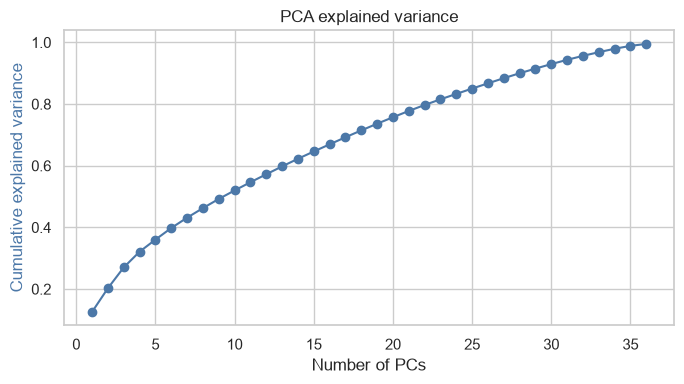
\includegraphics[width=.55\linewidth]{./figures/pca_expl_var.png}
  \caption{Cumulative explained variance (blue)  across all 37 principal components. }
  \label{fig:pca_spectrum}
\end{figure}

Next, we swept the perplexity parameter of \tsne{} \citep{maaten2008tsne} (via scikit-learn
\citep{pedregosa2011sklearn}) over the values 5, 15, 30, 40, 50, 60, 70 and 100, computing \trust{} and
\knnp{} on a fixed random subsample of 5{,}000 of our 40{,}000 balanced cells. \trust{} penalizes
embeddings that place points close together that were not close in the high-dimensional input, weighted
by how far out of the true neighbourhood a false neighbour originally ranked
\citep{venna2001trustworthiness}; \knnp{} is stricter, measuring the exact overlap of each point's $k$
nearest neighbours between the two representations, with no partial credit for a near-miss. \trust{}
scores in the range 50--100 were very similar (within about 0.0003), so we chose the marginal
maximum, 60 (\trust{}$=0.926$). Visually, perplexity 5 gives a largely undifferentiated cloud, while
higher perplexities show distinct clusters emerging (Supp.\ Fig.~\ref{fig:tsne}).

For UMAP \citep{mcinnes2018umap} we grid-searched learning rate ($0.1$, $0.5$, $1.0$, $5.0$), minimum
distance ($0.0$, $0.1$, $0.5$, $1$) and number of neighbours ($5$, $15$, $50$, $100$). The highest
\trust{} was obtained at learning rate $0.1$, 5 neighbours and minimum distance $0.0$
(Table~\ref{tab:umap_lr}, full grid in Supp.\ Fig.~\ref{fig:umap}). Visibly lower minimum distance packs points
more tightly and the number of neighbours changes cluster shape but has a smaller effect than minimum distance.

We compare these three methods using \trust{}, \knnp{} and the Pearson correlation ($r_d$) of all
pairwise distances. While the first two measures capture \emph{local} structure (is each point's immediate neighbourhood
preserved), $r_d$ captures \emph{global} structure (is the overall arrangement of near and far
points preserved, independent of exact neighbour identity). This distinction shows in the results (Table~\ref{tab:dr_comp}): \trust{} and \knnp{} agree on \tsne{} as the best method, but $r_d$ favours
PCA instead, consistent with PCA being a linear projection explicitly built to preserve variance/distance.

\begin{table}[h]
  \centering
  \begin{minipage}{0.62\linewidth}
    \centering
    {\footnotesize\begin{tabular}{lrrrr}\toprule
Embedding & $T(15)\uparrow$ & $R(15)\uparrow$ & $r_d\uparrow$ & $S_{\rm CMV}\uparrow$\\\midrule
PCA & \worst{0.7258} & \worst{0.0072} & \best{0.6204} & \worst{0.0016}\\
t-SNE & \best{0.9612} & \best{0.2232} & 0.4868 & 0.0104\\
UMAP & 0.9009 & 0.1126 & \worst{0.3954} & \best{0.0178}\\
\bottomrule\end{tabular}
}
    \caption{PCA, \tsne{} and UMAP: local structure via \trust{} ($T$) and \knnp{} ($R$), global
    structure via Pearson correlation ($r_d$) of pairwise distances. $T,R$ use $k=15$. Green: best per
    column; red: worst.}
    \label{tab:dr_comp}
  \end{minipage}
  \hfill
  \begin{minipage}{0.34\linewidth}
    \centering
    {\footnotesize\begin{tabular}{lrr}\toprule
Pair & $R(15)\uparrow$ & $M^2\downarrow$\\\midrule
PCA vs t-SNE & 0.00585 & \best{0.45189}\\
PCA vs UMAP & \worst{0.00410} & \worst{0.73390}\\
t-SNE vs UMAP & \best{0.12532} & 0.72369\\
\bottomrule\end{tabular}
}
    \caption{Pairwise \knnp{} ($R$, local) and Procrustes disparity ($M^2$, aligned global shape).}
    \label{tab:maps_comp}
  \end{minipage}
\end{table}

Finally, we compare each pair of methods using \knnp{} ($R$) and Procrustes disparity ($M^2$)
(Table~\ref{tab:maps_comp}). Procrustes disparity aligns two maps by translation/rotation/reflection/scaling, then measures the remaining mismatch after this optimal alignment;
a lower score means a closer overall shape once cosmetic differences in orientation and scale have been
removed \citep{scipy2020}.
By this measure, PCA and \tsne{} are the closest match, plausibly because our \tsne{} runs were PCA-initialized, seeding
its global layout before local optimization reshapes fine structure. By contrast, for local-neighbour
agreement ($R$), \tsne{} and UMAP are the more similar pair. The absolute $R$ values look small, but
chance level for $n=40{,}000$, $k=15$ is only $k/n\approx0.0004$, so even the smallest value is well
above chance.



\bibliographystyle{unsrtnat}
\bibliography{references}

\appendix
\section*{Supplementary Figures and Tables}

\begin{figure}[h]
  \centering
  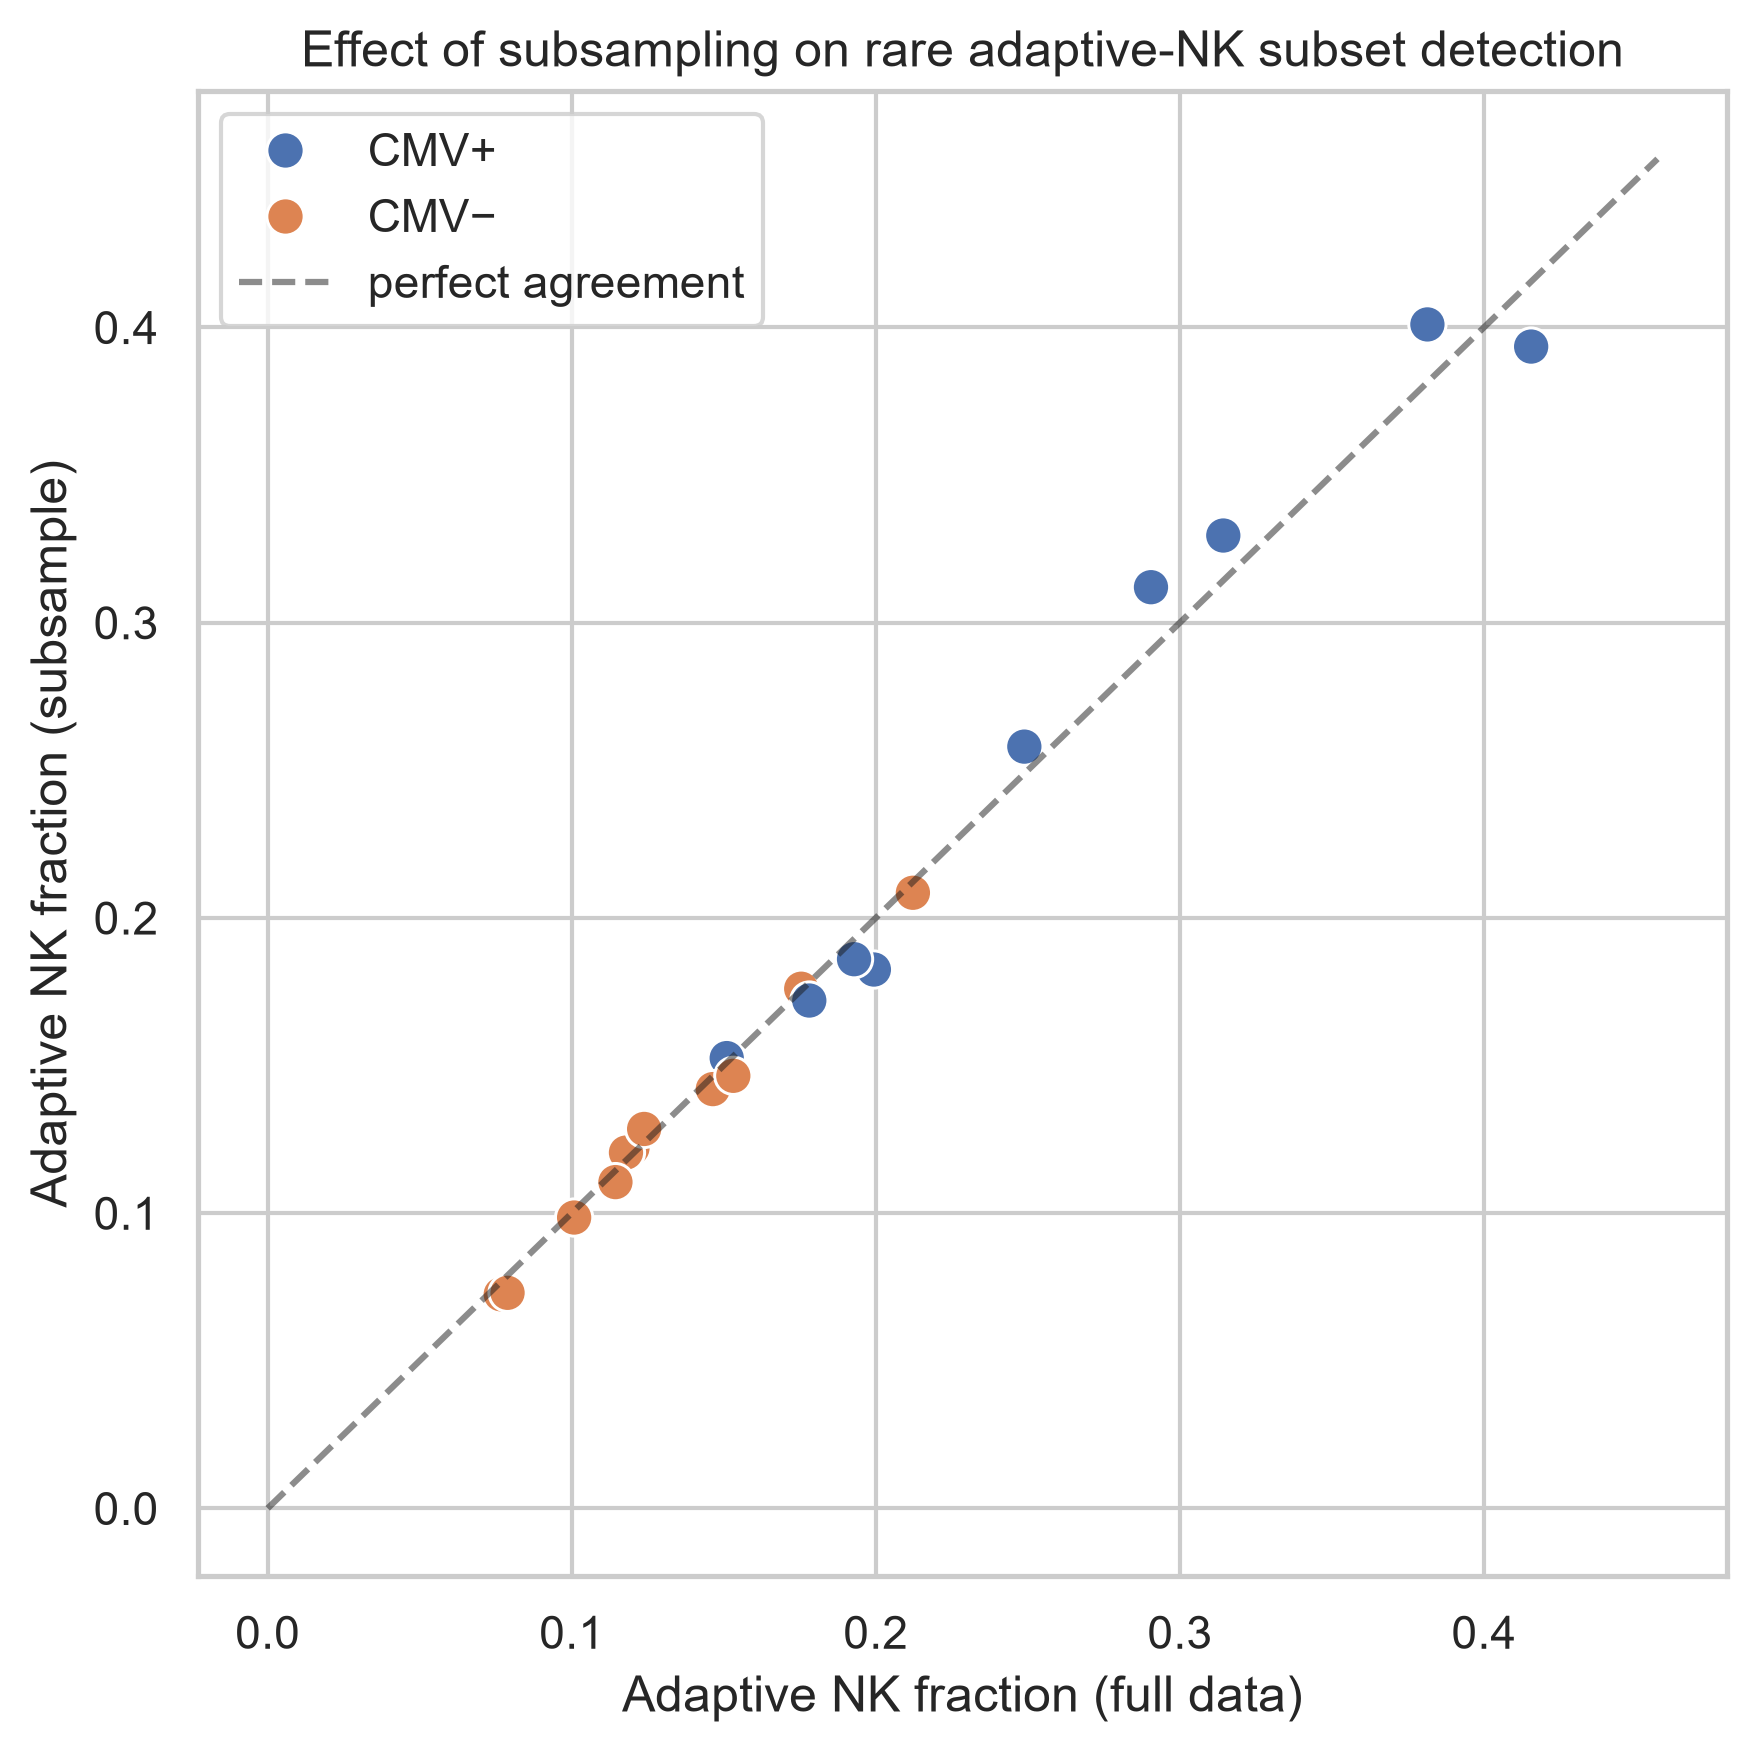
\includegraphics[height=50mm]{subsample.png}
  \caption{NKG2C$^+$/CD57$^+$ fraction, 2{,}000-cell subsample per donor vs.\ full population.}
  \label{fig:subsample}
\end{figure}

\begin{figure}[h]
  \centering
  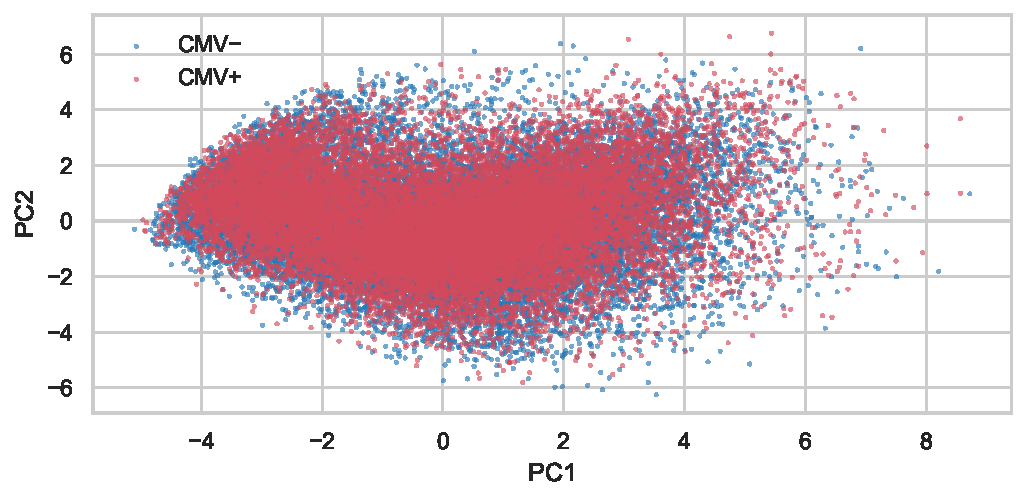
\includegraphics[width=.55\linewidth]{pca_donor.pdf}
  \caption{First two PCs, 40{,}000-cell sample, coloured by CMV status (CMV+: red, CMV$-$: blue).}
  \label{fig:pca_plot}
\end{figure}

\begin{figure}[h]
  \centering
  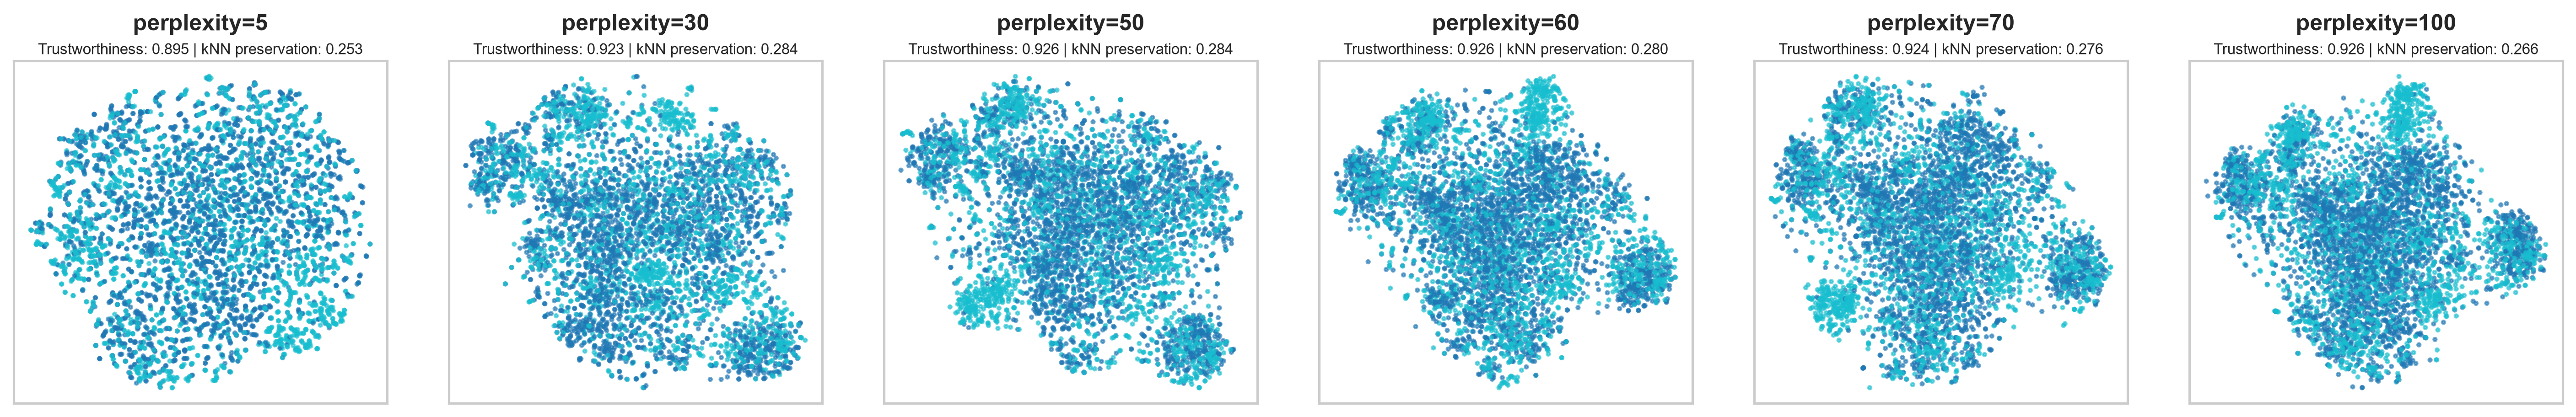
\includegraphics[width=\linewidth]{./figures/tsne_sweepp.png}
  \caption{\tsne{} embeddings, perplexities 5, 30, 50, 60, 70, 100; \trust{}/\knnp{} above each panel.}
  \label{fig:tsne}
\end{figure}

\begin{figure}[h]
  \centering
  
\includegraphics[width=.9\linewidth]{./figures/umap_sweep.png}
  \caption{UMAP grid: effect of $n_{\mathrm{neighbors}}$ and \texttt{min\_dist} at learning rate $0.1$.}
  \label{fig:umap}
\end{figure}

\begin{table}[h]
  \centering
  {\footnotesize
  \begin{tabular}{rrrrr}
    \toprule
    $\mathrm{learning\_rate}$ & $n_{\rm neighbors}$ & $\mathrm{min\_dist}$ & $T(15)\uparrow$ & $R(15)\uparrow$ \\
    \midrule
    0.1 & 5  & 0.0 & 0.895908 & 0.230373 \\
    0.5 & 5  & 0.0 & 0.893360 & 0.226933 \\
    1.0 & 5  & 0.0 & 0.890139 & 0.224227 \\
    5.0 & 5  & 0.0 & 0.878033 & 0.203747 \\
    0.1 & 50 & 0.1 & 0.864503 & 0.149040 \\
    0.5 & 50 & 0.1 & 0.862615 & 0.143093 \\
    1.0 & 50 & 0.1 & 0.856671 & 0.135920 \\
    5.0 & 50 & 0.1 & 0.840111 & 0.111320 \\
    \bottomrule
  \end{tabular}}
  \caption{Effect of UMAP learning rate on \trust{}/\knnp{} for two fixed (n\_neighbors, min\_dist) settings.}
  \label{tab:umap_lr}
\end{table}

\end{document}